 \subsection{Public Key Encryption Schemes}
Public crypto systems are good for key management, but they are slow.
They rely on mathematically difficult problems, which is why we need to use very
large numbers, which creates a lot computational overhead if you want to use them in practice. \\

IoT devices are increasingly used for cryptography because secure communication and data integrity 
are essential in IoT applications.
These devices often operate in environments where sensitive data is transmitted, requiring robust cryptographic mechanisms to ensure confidentiality, authentication, and integrity.
Public cryptographic systems face several challenges when implemented on IoT devices due to their unique constraints. These challenges include:
\begin{itemize}
    \item Resource constraints:
    \begin{itemize}
        \item \textit{Limited Processing Power:} IoT devices often lack sufficient computational capabilities for intensive cryptographic operations like RSA or ECC.
        \item \textit{Memory Limitations:} Minimal RAM and storage restrict the ability to handle large keys or certificates.
        \item \textit{Energy Consumption:} Asymmetric cryptography can deplete battery-powered devices quickly.
    \end{itemize}

    \item Network constraints:
    \begin{itemize}
        \item \textit{Bandwidth Limitations:} Low-bandwidth networks hinder the exchange of large cryptographic data.
        \item \textit{Latency Sensitivity:} Handshake protocols like TLS can increase latency, affecting real-time IoT applications.
    \end{itemize}

    \item Key management:
    \begin{itemize}
        \item \textit{Storage and Security:} Secure storage for keys is often unavailable.
        \item \textit{Scalability:} Managing keys for millions of devices is complex.
        \item \textit{Revocation and Updates:} Updating or revoking keys across many devices is challenging.
    \end{itemize}
    \item and much more...
\end{itemize}

\subsubsection{Goldwasser-Micali}
RSA is not IND-CPA secure (because it is deterministic). Attempt to have IND-CPA secure schemes based on factoring assumption:
GM is one such encryption. It is super expensive, because it encrypts a \emph{single} bit.
Not used in practice, but simple construction used to help build others. \\

GM is based on \textbf{QUADRES problem}: given a compositve integer $N$ and an integer $e$,
it is hard to test whether $e$ is a quadratic residue modulo $N$ or not.

\[ Q_N = \{x^2 \pmod{N} \ : x \in (\mathbb{Z}/N\mathbb{Z})^* \}, \]
\[ J_N = \{ a \in (\mathbb{Z}/N\mathbb{Z})^* \ : \left(\frac{a}{N}\right)=1\}\]

\[ N = p \cdot q\]

The size of $Q_N$ is $(p-1)(q-1)/4$ and the size of $J_N$ is $(p-1)(q-1)/2$. \\

\textbf{Key Generation:}
\[ N \leftarrow p \cdot q \]
\[ y \in J_N \backslash Q_N \]

\[ \text{private key} = (p,q) \]
\[ \text{public key} = (N,y) \]

How to find y?
\begin{enumerate}
    \item Pick $y_p$ in the finite field of prime numbers $p$: $y_p \in \mathbb{F}_p^*$
    \item Pick $y_q$ in the finite field of prime numbers $q$: $y_1 \in \mathbb{F}_q^*$
    \item Check if their Legendre symbols are $-1$: $\left(\frac{y_p}{p}\right) = \left(\frac{y_q}{q}\right) = -1$
    
    where the Legendre symbol is defined as:
    \[
    \left(\frac{a}{p}\right) =
    \begin{cases} 
    1 & \text{if } a \text{ is a quadratic residue mod } p \text{ and } a \neq 0, \\
    -1 & \text{if } a \text{ is a quadratic non-residue mod } p, \\
    0 & \text{if } a \equiv 0 \pmod{p}.
    \end{cases} \]
    
    So, a Legendre symbol of $-1$ indicates that the number is a quadratic non-residue modulo the respective prime.
    \item Use CRT to compute \( y \) modulo \( N \) (find an integer $y$ that satisfies the congruences): 
    \[
    y \equiv y_p \pmod{p}, \quad y \equiv y_q \pmod{q}.
    \]


    \item Compute the Jacobi symbol of \( y \) modulo \( N \) to ensure that \( y \) is in the set of Jacobi symbols \( J_N \) but not in the set of quadratic residues \( Q_N \):
    \[ \left(\frac{y}{N}\right) = \left(\frac{y}{p}\right) \cdot \left(\frac{y}{q}\right) =
    \left(\frac{y_p}{p}\right) \cdot \left(\frac{y_q}{q}\right) = (-1)\cdot(-1) = 1\] 

    A Jacobi symbol of 1 indicates that $y$is either a quadratic residue or a non-residue modulo $N$.
    However, since $y$ is constructed from non-residues modulo $p$ and $q$, it is specifically a quadratic non-residue modulo $N$.
\end{enumerate}

The selected \( y \) lies in the set of Jacobi symbols \( J_N \) ($=1$) but not in the set of quadratic residues \( Q_N \). 
This ensures that \( y \) has the desired cryptographic properties for use in the Goldwasser-Micali encryption scheme. \\

\textbf{Encryption and Decryption:}
Encrypt a single bit $b$:
\[ x \leftarrow \text{random} \in (\mathbb{Z}/N\mathbb{Z})^* \]
\[ c = y^b \cdot x^2\pmod{N} \]

For decrytion, compute the Jacobi symbol:
\[ \left(\frac{c}{p}\right) \]

If $b = 0$, then $c$ is a quadratic residue modulo $N$ and the Jacobi symbol is 1.
If $b = 1$, then $c$ is a quadratic non-residue modulo $N$ and the Jacobi symbol is -1. \\

\textbf{Security:}
\begin{itemize}
    \item GM is IND-CPA secure under the quadratic residuosity assumption. Ciphertexts are probabilistic.
    \item GM is \textbf{not} IND-CCA secure. In a CCA attack, an attacker can query a decryption oracle to learn about the plaintext corresponding to a ciphertext. 
    GM fails in this scenario because it is malleable, meaning an attacker can modify ciphertexts in ways that result in predictable changes to the decrypted message.
    \item GM is homomorphic because it supports additive operations on ciphertexts. Specifically, you can add two ciphertexts together and decrypt the result to get the sum of the corresponding plaintexts. 
    This malleability can be exploited in certain attacks, making the scheme unsuitable for applications requiring non-malleability (e.g., secure voting).
\end{itemize}

\subsubsection{ElGamal}
We want an encryption scheme that is IND-CPA secure and efficient.
ElGamal encryption uses domain paramaters
\begin{itemize}
    \item prime $p$ such that $p-1$ is divisible by another (large) prime $q$.
    Safe primes: $p = 2q + 1$
    \item generator $g$ is an element in finite field of $p$, with an of order $q$
\end{itemize}

\[ g = r^{(p-1)/q} \pmod{p} \neq 1 \ \text{for some} \ r \in \mathbb{F}_p^*\]

\textbf{Key Generation:}
\[ \text{private key}:  x \in [0, \cdots, q-1] \]
\[ \text{public key}: h \leftarrow g^x \pmod{p} \]

\textbf{Encryption and Decryption:}
To encrypt a message $m$ in $G$:    
\[ k \leftarrow \{0, \cdots, q-1\} \] 
\[ c_1 \leftarrow  g^k \]
\[ c_2 \leftarrow  m \cdot h^k \]

Output the ciphertext as $c \leftarrow (c_1, c_2) \in G\times G$. \\

To decrypt a ciphertext $c = (c_1, c_2)$:

\[ \frac{c_2}{c_1^x} = \frac{m \cdot h^k}{g^{x\cdot k}} = \frac{m \cdot g^{x\cdot k}}{g^{x\cdot k}} = m\] 

Recall: $h \leftarrow g^x \pmod{p}$, so $h^k = g^{x\cdot k} \pmod{p}$. \\

\textbf{Security:}
ElGamal is IND-CPA secure under the DDH assumption. But, still it is not IND-CCA secure.
This is because ElGamal is malleable (multiplicative homomorphic), meaning an attacker can modify ciphertexts in ways that result in predictable changes to the decrypted message.

\[ (c_1, c_2) = (g^k, m \cdot h^k) \]
\[ (c_1, 2\cdot c_2') =(g^k, 2\cdot m \cdot h^k)  \]

\subsubsection{Paillier}
Paillier encryption is a probabilistic asymmetric cryptographic scheme known for its \textbf{additive homomorphic properties}. It was introduced by Pascal Paillier in 1999 and is widely used in applications requiring secure computations on encrypted data, such as electronic voting and secure multiparty computation.
IND-CPA secure, efficient, and additively homomorphic encryption scheme.

\begin{thm}
    \textbf{Carmichael's Theorem:} Let $n = pq$ be a positive integer, where $p$ and $q$ are large numbers. $\phi(n)$ is Euler's 
    totient function and $\lambda(n) = \lcm(p-1, q-1)$. Then, for any $w \in \mathbb{Z}_{n^2}^*$, we have:
    \[ w^{\lambda} \equiv 1 \pmod{n} \]
    \[ w^{n\lambda} \equiv 1 \pmod{n^2} \]

\end{thm}

\begin{defn}
    The \textbf{Decisional Composite Residuosity Assumption} (DCRA) is a mathematical security assumption that underpins the Paillier encryption scheme. 
    Imagine you are given a random number $x$ and a composite number $N = pq$. 
    Can you tell if $x$ is a special kind of residue called an $N-th$ residue modulo $N^2$? \\


    An $\bold{N}$\textbf{-th residue modulo} $\bold{N^2}$ is a number that can be written in the form:

    \[ x = y^N \pmod{N^2} \]

    for some integer $y$. So, it's a number that was created by raising $y$ to $N$, then taking the remainder
    after dividing by $N^2$. 
    The DCRA states that it is computationally infeasible to distinguish between $N$-th residues and random numbers modulo $N^2$.
    Without the factorization of $N$, there is no efficient way to decide whether a given number is an $N$-th residue modulo $N^2$.
\end{defn}

The set of \( N \)-th residues modulo \( N^2 \) forms a subgroup of the multiplicative group \( \mathbb{Z}_{N^2}^* \). A generator \( g \in \mathbb{Z}_{N^2}^* \) ensures that these residues are well-structured and span the correct subgroup. Specifically:
\[
g^N \mod N^2
\]
is guaranteed to be an \( N \)-th residue, as it can be written as:
\[
g^N = (y^N) \mod N^2
\]
for some \( y \in \mathbb{Z}_{N^2}^* \). \\


\textbf{Key Generation:}
Let $n= pq$ and $g$ is a generator of group $\mathbb{Z}_{n^2}^*$ with an order of $n$. That is,
\[ g^n \equiv 1 \pmod{n^2} \]

$\lambda = \lcm(p-1, q-1)$ is the private key derived using the least common multiple.
The \textbf{secret key} is $(\lambda)$, and the \textbf{public key} is $(g,n)$. \\

\textbf{How to find such a generator $g$?} \\
\begin{align*}
    (1 + n) &\equiv 1 + n \pmod{n^2} \\
    (1 + n)^2 &\equiv 1 + 2n + n^2 \equiv 1 + 2n \pmod{n^2} \\
    (1 + n)^3 &\equiv 1 + 3n + 3n^2 + n^3 \equiv 1 + 3n \pmod{n^2} \\
    \vdots & \\
    (1 + n)^k &\equiv 1 + kn \pmod{n^2}
    \end{align*}
    Then:
    \[
    (1 + n)^n \equiv 1 + n \cdot n \equiv 1 \pmod{n^2}
    \]
    Thus:
    \[
    g = 1 + n
    \]

\textbf{Encryption and Decryption:}
For encryption, the input requires a random \( r \in \mathbb{Z}_N^* \) (a fresh random value for every encryption).
Then: 

\[ m \in \mathbb{Z}_n, \ r \in_R \mathbb{Z}_n^* \]

\[ E_{pk}(m) = g^m \cdot r^N \mod N^2 \] 


where \( g^m \) encodes the message \( m \), and \( r^N \) adds randomness to ensure probabilistic encryption (different ciphertexts for the same \( m \)). \\

For decryption, the private key \( \lambda \) is used to recover the plaintext \( m \) from the ciphertext \( c \):

\[
D_{sk}(c) = \frac{L(c^\lambda \mod n^2)}{L(g^\lambda \mod n^2)} \mod n \quad \text{where } L(u) = \frac{u - 1}{n}
\]

Why does it work? \\
\begin{align*}
c^\lambda \mod n^2 &= (g^m r^n)^\lambda = g^{m\lambda} r^{n\lambda} \mod n^2 \\
&= (1 + n)^m r^{n\lambda} \mod n^2 = 1 + nm\lambda. \\
g^\lambda \mod n^2 &= (1 + n)^\lambda = 1 + n\lambda. \\
\frac{L(1 + nm\lambda)}{L(1 + n\lambda)} &= \frac{m\lambda}{\lambda} \mod n \equiv m \mod n.
\end{align*}

\( c^\lambda \mod N^2 \) removes the random component \( r^N \), isolating \( g^m \).

\subsubsection{Additive Homomorphism}
Homomorphism:

\[ E_{pk}(m_1) \otimes E_{pk}(m_2) = E_{pk}(m_1 \oplus m_2) \]

Additive homomorphism:
\[ E_{pk}(m_1) \times E_{pk}(m_2) = E_{pk}(m_1 + m_2) \]
\[ \underbrace{E_{pk}(m) \times E_{pk}(m) \cdots E_{pk}(m)}_{\text{c times}}  = E_{pk}(m)^c = E_{pk}(m \cdot c) \]

The key feature of Paillier encryption is its \textbf{additive homomorphism}, meaning:

\[
c_1 = g^{m_1} \cdot r_1^N \mod N^2, \quad c_2 = g^{m_2} \cdot r_2^N \mod N^2
\]
When \( c_1 \cdot c_2 \mod N^2 \) is computed, the result is:
\[
c = c_1 \cdot c_2 \mod N^2 = g^{m_1 + m_2} \cdot (r_1 \cdot r_2)^N \mod N^2
\]
Decrypting \( c \) yields \( m_1 + m_2 \mod N \), enabling computations on encrypted data.

\Comment{explain more? i dont think we need to know this in this much detail}


\subsubsection{RSA-OAEP}
RSA is not IND-CPA secure, thus we need redudancy. Padding can help, but this should be random.

\begin{defn}
    \textbf{Optimal Asymmetric Encryption Padding} (OAEP) is a cryptographic padding scheme used in public-key encryption systems, 
    such as RSA, to enhance security. It ensures that the encryption process introduces randomness and 
    prevents certain types of attacks, such as chosen-plaintext attacks.
    OAEP combines the original message with a random value and uses a series of cryptographic functions 
    (such as hash functions and a mask generation function) to transform the message into a padded format.
\end{defn}

Let $f$ be any $k$-bit to $k$-bit trapdoor one-way permutation.
Let $k_0$ and $k_1$ be numbers such that the effort of $2^{k_0}$ and $2^{k_1}$ is impossible, i.e., $k_0, k_1 > 128$ bits.
Let $n$ be $k-k_0-k_1$. Define the following hash functions:

\[ G: \{0,1\}^{k_0} \times \{0,1\}^n \rightarrow \{0,1\}^{n+ k_1} \]
\[ H: \{0,1\}^{n+k_1} \rightarrow \{0,1\}^{k_0} \]

\begin{figure}[h!]
    \centering
    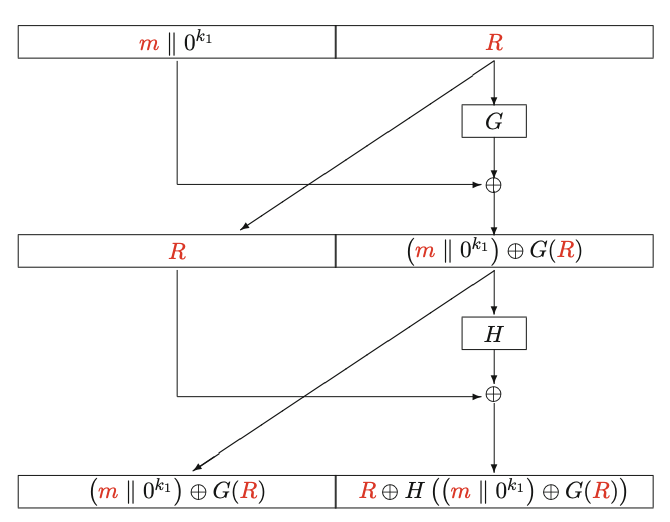
\includegraphics[width=0.35\textwidth]{img/oaep.png}
    \caption{OAEP as a Feistel network}
    \label{fig:oaep}
\end{figure}

Let $m$ be a message of size $n$ bits. The OAEP encryption scheme is as follows:

\[ c \leftarrow E(m) = f \left( \left\{ (m || 0^{k_1}) \oplus G(R) \right\}
|| \left\{ R \otimes H((m || 0^{k_0})\oplus G(R))\right\}\right) = f(A)\]

where $R$ is a random $k_0$-bit string, $||$ is concatenation, and $m || 0^{k_1}$ means $m$
followed by $k_1$ zero bits. \\

To decrypt, apply the trapdoor to $f$ to recover $A$:
\[ A = f^{-1}(c) = \{ T || \{R \oplus H(T) \} \} \]
Compute $H(T)$ and recover $R$ from $R \oplus H(T)$. 
Then, compute $G(R)$ and recover $v = m || 0^{k_1} = (m || 0^{k_1}) \oplus G(R)$.
If $v$ ends in $k_1$ zeros, then $m$ is the output message. Otherwise, the decryption fails. \\

In the Random Oracle Model (ROM), if $G$ and $H$ are secure, then RSA-OAEP is IND-CCA secure.

\subsubsection{Fujisaki-Okamoto Transform}
The \textbf{Fujisaki-Okamoto transform} is a technique used to enhance the security of encryption schemes, 
particularly in public-key cryptography,
by converting a semantically secure encryption scheme into one that 
is secure against chosen ciphertext attacks.
Obtain IND-CCA secure schemes from IND-CPA secure schemes (add randomness, destroy homomorphism).
The transform involves adding randomness and applying a second encryption operation on the ciphertext.\\

It is simple and elegant: 
\[ \text{original scheme:} \quad E(m,r) \]
\[ \text{new scheme:} \quad E'(m,r) = E(m ||r, H(m||r)) \]

where $r$ is randomness, and $H$ is a hash function. \\

\textbf{Key Idea:}
It uses a hash function to derive a \textbf{mask}, which is then used to modify the ciphertext. 
This prevents attackers from gaining any useful information even if they have access to a decryption oracle 
(which lets them decrypt chosen ciphertexts). \\

\textbf{Example:}
\[ E(m,r) = (g^r, m \cdot h^r) \]
(ElGamal encryption) \\

\[ E' = (g^{H(m||r)}, (m ||r)\cdot h^{H(m||r)}) \]

\[ c = E(m', H(m'))\]

Other transforms exist.

\subsection{Hybrid Ciphers}
Symmetric key algoritums are fast bu have the key distribution problem. Assymetric key algorithms
are slow, but key distribution is easier. In practice, KEM/DEM approach is used:

\begin{itemize}
    \item Encrypt the data using a symmetric cipher
    \item Send the encryption key using an asymmetric cipher
\end{itemize}

KEM = Key Encapsulation Mechanism. Has a public key component.
DEM = Data Encapsulation Mechanism. Has a private key component. \\

To \textbf{encrypt} a message \( m \) to a user with \( (pk, sk) \):

\begin{itemize}
    \item \( (k, c_1) \leftarrow \text{Encap}_{\mathcal{pk}}() \): Generate a random key \( k \) and encapsulate it into \( c_1 \).
    \item \( c_2 \leftarrow e_k(m) \): Encrypt the message \( m \) using the key \( k \) to get \( c_2 \).
    \item \( c \leftarrow (c_1, c_2) \): The ciphertext \( c \) is the combination of \( c_1 \) and \( c_2 \).
\end{itemize}

Upon receiving the ciphertext \( c \), the recipient can \textbf{decrypt} it as follows:

\begin{itemize}
    \item \( k \leftarrow \text{Decap}_{\mathcal{sk}}(c_1) \): Decapsulate \( k \) from \( c_1 \) using the secret key \( \mathcal{sk} \).
    \item If \( k = \bot \), then output \( \bot \).
    \item \( m \leftarrow d_k(c_2) \): Decrypt \( c_2 \) using the key \( k \) to get the message \( m \).
    \item Return \( m \).
\end{itemize}

Given that KEM and DEM are \textbf{secure separate}, the hybrid system is secure as well.

\begin{figure}[h!]
    \centering
    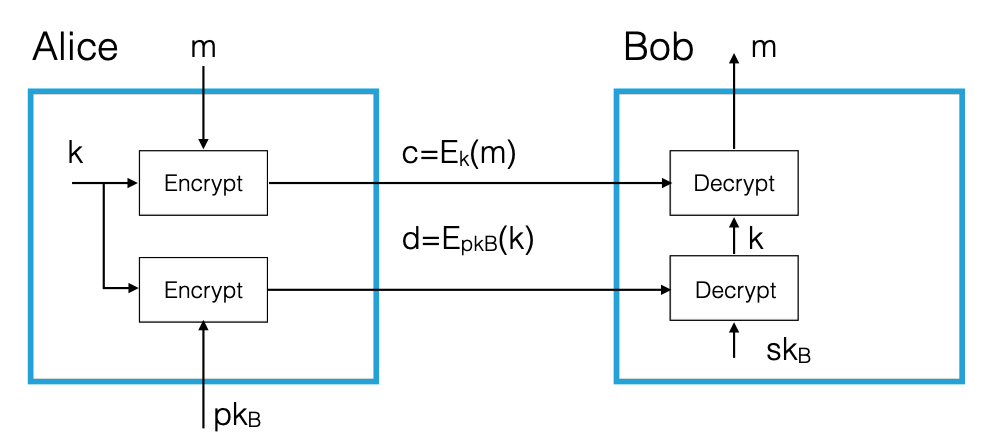
\includegraphics[width=0.5\textwidth]{img/securecom.png}
    \caption{Secure Communication}
\end{figure}

\subsubsection{RSA-KEM}
Let $N$ be the RSA modulus, the product of two primes $p$ and $q$.
The function $f$ is the encryption algorithm for RSA.
Then, encapsulation works as follows:

\begin{itemize}
    \item $x \leftarrow \{1, cdots, N-1 \}$
    \item $c \leftarrow f_{N,e}(x)$
    \item $k \leftarrow H(x)$
    \item Output is $(k,c)$
\end{itemize}

Dececapsulation works as follows, performed by the holder of the secret key:

\begin{itemize}
    \item $x \leftarrow f_{N}^{-1}(c)$
    \item $k \leftarrow H(x)$
    \item Output is $k$
\end{itemize}

RSA-KEM is IND-CCA secure under ROM.

\subsubsection{DHIES-KEM}
Diffie-Hellman Integrated Encryption Scheme. \\

\textbf{Key Generation:}
\begin{itemize}
    \item A cyclic finite abelian group $G$ of prime order $q$
    \item A generator $g$ of $G$
    \item Key space $K$
    \item A key derivation function $H$
    \item Generate $x \in \mathbb{Z}/q\mathbb{Z}$
    \item Compute $h = g^x$
\end{itemize}

For \textbf{encapsulation}, the sender does the following:
\begin{itemize}
    \item \( u \leftarrow \mathbb{Z}/q\mathbb{Z} \): Generate a random value \( u \) from the group \( \mathbb{Z}/q\mathbb{Z} \).
    \item \( v \leftarrow h^u \): Compute \( v \) by raising \( h \) (from the key generation) to the power of \( u \), producing a value in the group \( G \).
    \item \( c \leftarrow g^u \): Compute \( c \) by raising the generator \( g \) to the power of \( u \), which will be sent as part of the ciphertext.
    \item \( k \leftarrow H(v \parallel c) \): Use a key derivation function \( H \) to derive a shared key \( k \) by applying \( H \) to the concatenation of \( v \) and \( c \).
\end{itemize}

For \textbf{decapsulation}, the recipient does the following:
\begin{itemize}
    \item \( v \leftarrow c^x \): Compute \( v \) by raising the received ciphertext \( c \) to the power of the secret key \( x \).
    \item \( k \leftarrow H(v || c) \): Use the key derivation function \( H \) to derive the shared key \( k \) by applying \( H \) to the concatenation of \( v \) and \( c \).
\end{itemize}

This scheme is IND-CCA secure under ROM.

\subsection{Secure Digital Signatures} 

\subsubsection{RSA-FDH}
\textbf{RSA-FDH (Full Domain Hash)} is a cryptographic signature scheme that combines the RSA algorithm with the concept of hashing 
to ensure the security and integrity of digital signatures.
RSA and hash functions (such as SHA-256) can be combined for an efficient and secure signature scheme.

\begin{enumerate}
    \item Take a message $m$ and compute the hash $h = H(m)$
    \item Sign the hash $h$ using the RSA private key $d$ to get the signature $s = h^d \mod N$
    \item Compute $h' = H(m)$ upon receiving the message $m$
    \item Verify the signature using the pulic key and obtain $h$ using $s^e \mod N$
    \item Compare if the two hashes $h = h'$ match
\end{enumerate}

This scheme is secure, however, the codomain of the hash function should match the domain of RSA. This is not possible in practice, so we use the RSA-PSS scheme.

\subsubsection{RSA-PSS}
\textbf{RSA-PSS (Probabilistic Signature Scheme)} is a secure digital signature scheme that combines the RSA algorithm with the Probabilistic Signature Scheme (PSS) padding scheme. \\

N is an RSA modulo is size $k$ bits, with $e$ and $d$ as the public and private exponents.
Define two parameters $k_0$ and $k_1$ such that $k_0 + k_1< k -1 $.
Define the following hash functions:

\[ G: \{0,1\}^{k_2}  \rightarrow \{0,1\}^{k - k_1 -1} \]
\[ H: \{0,1\}^* \rightarrow \{0,1\}^{k_1} \]

and

\[ G_1: \{0,1\}^{k_1}  \rightarrow \{0,1\}^{k_0} \]
\[ G_2: \{0,1\}^{k_1}  \rightarrow \{0,1\}^{k - k_0 - k_1 -1} \]
\[ G(w) = G_1(w) || G_2(w)\]

\textbf{Signing:} To sign a message $m$, the private key holder performs:
\begin{itemize}
    \item $r \leftarrow \{0,1\}^{k_0}$
    \item $w \leftarrow H(m||r)$
    \item $y \leftarrow 0||w||(G_1(w)\oplus r)||G_2(w)$
    \item $s \leftarrow y^d \pmod{N}$
\end{itemize}

\textbf{Verification:} To verify a signature $s$ on a message $m$ ($(s,m)$), the public key holder performs:
\begin{itemize}
    \item $y \leftarrow s^e \pmod{N}$
    \item Split $y$ into the components 
    \[ b||w||\alpha||\gamma\]
    where $b$ is one bit long, $w$ is $k_1$ bits long, $\alpha$ is $k_0$ bits long, and $\gamma$ is $k - k_0 - k_1 -1$ bits long.

    \item Compute $r = \alpha \oplus G_1(w)$
    \item The signature is verified as correct if and only if $b = 0$, $G_2(w) = \gamma$, and $H(m||r) = w$.
\end{itemize}

\subsubsection{The Digital Signature Algorithm (DSA)}
Reasons to have a DSA:
\begin{itemize}
    \item RSA based schemes are costly in terms of signature generation
    \item RSA based signatures are large
    \item RSA might be broken soon
\end{itemize}

DSA is based on finite fielsds or elliptic curves (EC-DSA).

\begin{figure}[h!]
    \centering
    \begin{subfigure}[t]{0.3\textwidth}
        \centering
        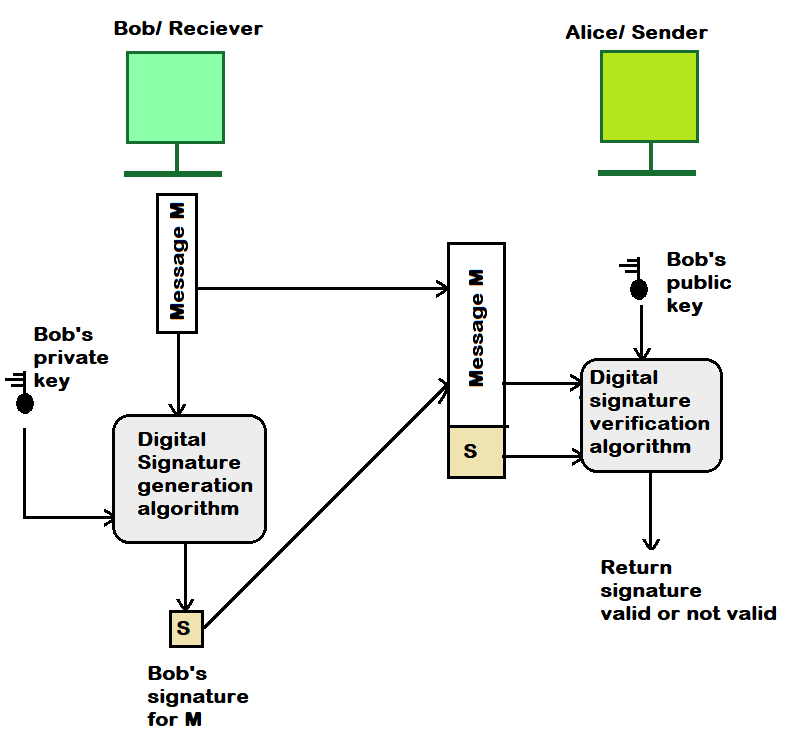
\includegraphics[width=\textwidth]{img/digsign.png}
        \caption{Model of Digital Signature Process}
    \end{subfigure}
    \hspace{0.1\textwidth}
    \begin{subfigure}[t]{0.5\textwidth}
        \centering
        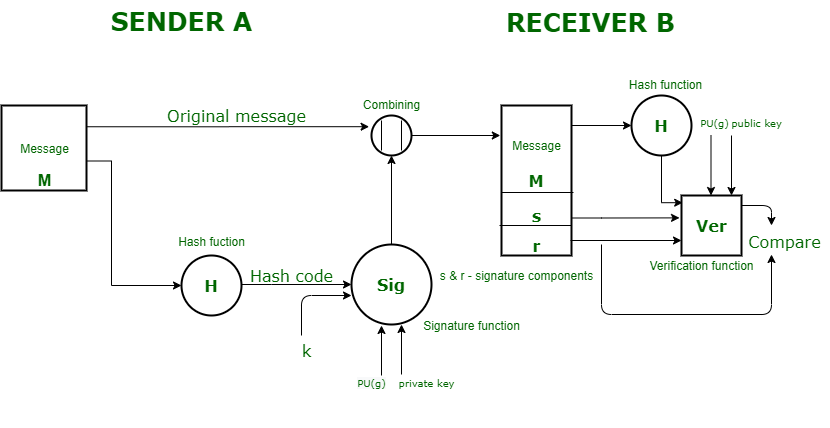
\includegraphics[width=\textwidth]{img/dsa.png}
        \caption{DSA Approach. PU$_G$ = global public key}
    \end{subfigure}
    \caption{Digital Signature Models}
    \label{fig:digsign-dsa}
\end{figure}

\textbf{Parameters:}
\begin{itemize}
    \item A large prime $p$ such that $p-1$ is divisible by a another (large) prime $q$
    \item A generator $g$ of the field in $\mod p$, with an order $q$ in $\mathbb{Z}_p^*$
    \item A hash function $H$ that maps bit strings to $Z/pZ$
    \item DSA works in the cyclic subgroup of size $q$, where $q > 256$ bits (for 128 bit security) and $p > 2048$ bits
\end{itemize}

\textbf{Key Generation:}
\begin{itemize}
    \item Generate a private key $x \in \{1, \cdots, q-1\}$
    \item Compute the public key $h = g^x \mod p$, where $h$ is the public key
\end{itemize}

\textbf{Signing:} Sign with private key. Compute the signature $(s, r)$ on a message $m$ in $Z/qZ$:
\begin{itemize}
    \item $h \leftarrow H(m)$:
    \begin{itemize}
        \item Compute the cryptographic hash $h$ of the message $m$ using the hash function $H$.
    \end{itemize}
    \item $k \leftarrow (Z/qZ)^*$:
    \begin{itemize}
        \item Select a random integer $k$ from the set $(Z/qZ)^*$, which includes all integers modulo $q$ excluding zero.
        \item The value of $k$ must be kept secret and should not be reused for multiple signatures, as reusing $k$ can lead to the recovery of the private key $x$.
        \item $k$ is used to produce the signature components $r$ and $s$. 
    \end{itemize}
    \item $r \leftarrow (g^k \pmod{p}) \pmod{q}$:
    \begin{itemize}
        \item Compute the value of $r$ by raising the generator $g$ to the power of $k$, taking the result modulo $p$, and then reducing modulo $q$.
        \item The value $r$ depends on the random value $k$ and the group parameters $p$, $q$, and $g$.
        \item This step ensures that $r$ is deterministic for a given $k$, while remaining unpredictable due to the randomness of $k$.
    \end{itemize}
    \item $s \leftarrow (h + x \cdot r) \backslash k \pmod{q}$:
    \begin{itemize}
        \item Compute $s$ by first calculating $(h + x \cdot r) \mod q$, where $x$ is the private key and $h$ is the hash of the message.
        \item The value $s$ incorporates the message hash $h$, the private key $x$, and the randomness of $k$, binding the signature to both the message and the signer.
    \end{itemize}
\end{itemize}

\textbf{Verification:} Verify with public key (derived from private key and shared publicly).
To verify a signature $(s,r)$ on a message $m$, using the public key $h$:
\begin{itemize}
    \item To verify the signature \((r, s)\), the verifier uses the global parameters (\(p\), \(q\), \(g\)), the sender's public key \(y\), and the message hash \(h = H(m)\).
    \item $h \leftarrow H(m)$: The receiver computes the hash of the received message $m$
    \item $a \leftarrow h / s \pmod{q}$, where $h = H(m)$. 
    \(a\) represents a part of the verification equation tied to the message hash and the signature.
    \item $b \leftarrow r / s \pmod{q}$. 
    \(b\) accounts for the contribution of the signature component \(r\) in the verification process.
    Together, \(a\) and \(b\) serve as inputs to reconstruct the expected value of the signature.
    \item $v \leftarrow (g^a \cdot h^b \pmod{p}) \pmod{q}$, where $h$ is the \textbf{public key}.
    Compute \(v\) as the combination of \(g^a\) and \(y^b\), reduced modulo \(p\) and \(q\).  
    \begin{itemize}
        \item \(g^a \mod p\): Represents the contribution of the message hash \(h\) scaled by the random value \(k\).
        \item \(y^b \mod p\): Represents the contribution of the public key \(y\), derived from the private key \(x\).
    \end{itemize}

    \item Accept the signature if and only if $v = r$.
    This final check ensures that the signature \((r, s)\) corresponds to the message \(m\) and the signer’s private key \(x\), without revealing \(x\).
\end{itemize}

DSA is slower than RSA. Operations over 2048 bit values, and they are expensive, since inverses have to be computed

\subsubsection{EC-DSA}
\textbf{Elliptic Curve Digital Signature Algorithm} is an elliptic curve-based variant of DSA,
designed to provide equivalent security to DSA but with smaller key sizes, making it more efficient for computation, storage, and bandwidth. \\

Choose a random integer $a$ and a point $P$ on the curve. The private key is $a$ and the public key is $Q = aP$. \\

\textbf{Signing:}
\begin{itemize}
    \item Choose a random number $k$
    \item Compute $kP = (x_1, y_1)$
    \item Compute $s = k^{-1}(H(m) + ax_1)$
    \item Signature is $(x_1, s)$
\end{itemize}

\textbf{Verification:}
\begin{itemize}
    \item Compute $u_1 = H(m)s^{-1}$ and $u_2 = x_1s^{-1}$
    \item Compute $u_1P + u_2Q = (x_0, y_0)$
    \item Check if $x_0 = x_1$
\end{itemize}

Remark:
\[ u_1P = u_2Q = u_1P + u_2aP = P(u_1 + u_2a) \]
\[ = P(H(m)s^{-1} + x_1s^{-1}a) = P(H(m)s^{-1} + k - H(m)s^{-1}) = kP\]

This demonstrates the relationship between the elliptic curve point \(P = u_1G + u_2Q\) and the random value \(k\) used during signing, where:
    \[
    P = u_1G + u_2Q = kP
    \]
During verification, \(P\) is calculated using the signature components \(r\) and \(s\), the message hash \(H(m)\), and the public key \(Q\).
 By substituting the definitions of \(u_1 = H(m)s^{-1} \mod n\) and \(u_2 = rs^{-1} \mod n\), the equation becomes:
    \[
    P = G(s^{-1}(H(m) + rd))
    \]

    The term \(H(m) + rd\) matches the signature equation, where:
    \[
    H(m) + rd = ks
    \]
    Substituting this gives:
    \[
    P = G(k) = kG
    \]

    This shows that the point \(P\) calculated during verification is equal to the point \(kP\) generated during the signing process, ensuring the correctness of the signature.





\subsubsection{Comparison of RSA, DSA, and ECDSA}
\begin{itemize}
    \item \textbf{Speed for digital signature:} RSA is better than DSA or ECDSA.
    \item \textbf{Key size:} EC-DSA requires smaller key sizes than RSA or DSA.
    \item \textbf{Implementation:} EC-DSA is easier to implement than DSA or RSA.
\end{itemize}

\subsubsection{Schorr Signatures}
\Comment{do we really need to know these two?}
\subsubsection{Nyberg-Rueppel Signatures}